\chapter{Frequently Asked Questions}
\label{ch:faq}

This chapter provides answers to some of the most frequently asked questions concerning usage, configuration and extension of the \apsq framework.

\section{Installation \& Usage}

\begin{description}
\item[What is the easiest way to use \apsq on CERN's LXPLUS?]
Central installations of \apsq on LXPLUS are provided via CVMFS for both supported LXPLUS operating systems, SLC6 and CERN CentOS7. Please refer to Section~\ref{sec:cvmfs} for the details of how to access these installations.
\item[What is the quickest way to get a local installation of \apsq?]
The project provides ready-to-use Docker containers which contain all dependencies such as Geant4 and ROOT. Please refer to Section~\ref{sec:docker} for more information on how to start and use these containers.
\end{description}

\section{Configuration}
\begin{description}
\item[How do I run a module only for one detector?]
This is only possible for detector modules (which are constructed to work on individual detectors).
To run it on a single detector, one should add a parameter \parameter{name} specifying the name of the detector (as defined in the detector configuration file):
\begin{minted}[frame=single,framesep=3pt,breaklines=true,tabsize=2,linenos]{ini}
[ElectricFieldReader]
name = "dut"
model = "init"
file_name = "../example_electric_field.init"
\end{minted}
\item[How do I run a module only for a specific detector type?]
This is only possible for detector modules (which are constructed to work on individual detectors).
To run it for a specific type of detector, one should add a parameter \parameter{type} with the type of the detector model (as set in the detector configuration file by the \parameter{model} parameter):
\begin{minted}[frame=single,framesep=3pt,breaklines=true,tabsize=2,linenos]{ini}
[ElectricFieldReader]
type = "timepix"
model = "linear"
bias_voltage = -50V
depletion_voltage = -30V
\end{minted}
Please refer to Section~\ref{sec:module_instantiation} for more information.
\item[How can I run the exact same type of module with different settings?] This is possible by using the \parameter{input} and \parameter{output} parameters of a module that specify the messages of the module:
\begin{minted}[frame=single,framesep=3pt,breaklines=true,tabsize=2,linenos]{ini}
[DefaultDigitizer]
name = "dut0"
adc_resolution = 4
output = "low_adc_resolution"

[DefaultDigitizer]
name = "dut0"
adc_resolution = 12
output = "high_adc_resolution"
\end{minted}
By default, both the input and the output of module are messages with an empty name.
In order to further process the data, subsequent modules require the \parameter{input} parameter to not receive multiple messages:
\begin{minted}[frame=single,framesep=3pt,breaklines=true,tabsize=2,linenos]{ini}
[DetectorHistogrammer]
input = "low_adc_resolution"
name = "dut0"

[DetectorHistogrammer]
input = "high_adc_resolution"
name = "dut0"
\end{minted}
Please refer to Section~\ref{sec:objects_messages} for more information.
\item[How can I temporarily ignore a module during development?]
The section header of a particular module in the configuration file can be replaced by the string \parameter{Ignore}.
The section and all of its key/value pairs are then ignored.
Modules can also be excluded from the compilation process as explained in Section~\ref{sec:cmake_config}.
\item[Can I get a high verbosity level only for a specific module?]
Yes, it is possible to specify verbosity levels and log formats per module.
This can be done by adding the \parameter{log_level} and/or \parameter{log_format} key to a specific module to replace the parameter in the global configuration sections.

\item[Can I import an electric field from TCAD and use it for simulating propagation?]
Yes, the framework includes a tool to convert DF-ISE files from TCAD to an internal format which \apsq can parse.
More information about this tool can be found in Section~\ref{sec:tcad_electric_field_converter}, instructions to import the generated field are provided in Section~\ref{sec:module_electric_field}.
\end{description}

\section{Detector Models}
\begin{description}
\item[I want to use a detector model with one or several small changes, do I have to create a whole new model for this?] No, models can be specialized in the detector configuration file.
To specialize a detector model, the key that should be changed in the standard detector model, e.g.\ like \parameter{sensor_thickness}, should be added as key to the section of the detector configuration (which already contains the position, orientation and the base model of the detector).
Only parameters in the header of detector models can be changed.
If support layers should be changed, or new support layers are needed, a new model should be created instead.
Please refer to Section~\ref{sec:detector_models} for more information.
\end{description}

\section{Data Analysis}
\begin{description}
\item[How do I access the history of a particular object?]
Many objects can include an internal link to related other objects (for example \parameter{getPropagatedCharges} in the \parameter{PixelCharge} object), containing the history of the object (thus the objects that were used to construct the current object).
These referenced objects are stored as special ROOT pointers inside the object, which can only be accessed if the referenced object is available in memory.
In \apsq this requirement can be automatically fulfilled by also binding the history object of interest in a module.
During analysis, the tree holding the referenced object should be loaded and pointing to the same event entry as the object that requests the reference.
If the referenced object can not be loaded, an exception is thrown by the retrieving method.
Please refer to Section~\ref{sec:objhistory} for more information.
\item[How do I access the Monte Carlo truth of a specific PixelHit?]
The Monte Carlo truth is part of the history of a PixelHit.
This means that the Monte Carlo truth can be retrieved as described in the question above.
Because accessing the Monte Carlo truth of a PixelHit is quite a common task, these references are stored directly for every new object created.
This allows to retain the information without the necessity to keep the full object history including all intermediate steps in memory.
Please refer to Section~\ref{sec:objhistory} for more information.
\item[How do I find out, which Monte Carlo particles are primary particles and which have been generated in the sensor?]
The Monte Carlo truth information is stored per-sensor as MCParticle objects. Each MCParticle stores, among other information, a reference to its parent. Particles which have entered the sensor from the outside world do not have parent MCParticles in the respective sensor and are thus primaries.

Using this approach it is possible, to e.g.\ treat a secondary particle produced in one detector as primary in a following detector.

Below is some pseudo-code to filter a list of MCParticle objects for primaries based on their parent relationship:

\begin{minted}[frame=single,framesep=3pt,breaklines=true,tabsize=2,linenos]{c++}
// Collect all primary particles of the event:
std::vector<const MCParticle*> primaries;

// Loop over all MCParticles available
for(auto& mc_particle : my_mc_particles) {
    // Check for possible parents:
    if(mc_particle.getParent() != nullptr) {
        // Has a parent, thus was created inside this sensor.
        continue;
    }

    // Has no parent particles in this sensor, add to primary list.
    primaries.push_back(&mc_particle);
}
\end{minted}

A similar function is used e.g.\ in the DetectorHistogrammer module to filter primary particles and create position-resolved graphs.
\end{description}

\section{Development}
\begin{description}
\item[How do I write my own output module?]
An essential requirement of any output module is its ability to receive any message of the framework.
This can be implemented by defining a private \command{listener} function for the module as described in Section~\ref{sec:objects_messages}.
This function will be called for every new message dispatched within the framework, and should contain code to decide whether to discard or cache a message for processing.
Heavy-duty tasks such as handling data should not be performed in the \command{listener} routine, but deferred to the \command{run} function of the respective output module.

\item[How do I process data from multiple detectors?]
When developing a new \apsq module which processes data from multiple detectors, e.g.\ as the simulation of a track trigger module, this module has to be of type \emph{unqiue} as described in Section~\ref{sec:module_manager}.
As a \emph{detector} module, it would always only have access to the information linked to the specific detector is has been instantiated for.
The module should then request all messages of the desired type using the messenger call \command{bindMulti} as described in Section~\ref{sec:objects_messages}.
For \emph{PixelHit} messages, an example code would be:

\begin{minted}[frame=single,framesep=3pt,breaklines=true,tabsize=2,linenos]{c++}
TrackTriggerModule(Configuration&, Messenger* messenger, GeometryManager* geo_manager) {
    messenger->bindMulti(this,
                         &TrackTriggerModule::messages,
                         MsgFlags::NONE);
}
std::vector<std::shared_ptr<PixelHitMessage>> messages;
\end{minted}
The correct detectors have then to be selected in the \command{run} function of the module implementation.
\item[How do I calculate an efficiency in a module?]
Calculating efficiencies always requires a reference.
For hit detection efficiencies in \apsq, this could be the Monte Carlo truth information available via the \emph{MCParticle} objects.
Since the framework only runs modules, if all input message requirements are satisfied, the message flags described in Section~\ref{sec:messageflags} have to be set up accordingly.
For the hit efficiency example, two different message types are required, and the Monte Carlo truth should always be required (using \command{MsgFlags::REQUIRED}) while the \emph{PixelHit} message should be optional:
\begin{minted}[frame=single,framesep=3pt,breaklines=true,tabsize=2,linenos]{c++}
MyModule::MyModule(Configuration& config, Messenger* messenger, std::shared_ptr<Detector> detector)
    : Module(config, detector), detector_(std::move(detector)) {

    // Bind messages
    messenger->bindSingle(this, &MyModule::pixels_message_);
    messenger->bindSingle(this, &MyModule::mcparticle_message_, MsgFlags::REQUIRED);
}
\end{minted}
\end{description}

\section{Miscellaneous}
\begin{description}
\item[How can I produce nicely looking drift-diffusion line graphs?]
The GenericPropagation module offers the possibility to produce line graphs depicting the path each of the charge carrier groups have taken during the simulation. This is a very useful way to visualize the drift and diffusion along field lines.

An optional parameter allows to reduce the lines drawn to those charge carrier groups which have reached the sensor surface to provide some insight into where from the collected charge carriers originate and how they reached the implants.
One graph is written per event simulated, usually this option should thus only be used when simulating one or a few events but not during a production run.

In order to produce a precise enough line graph, the integration time steps have to be chosen carefully - usually finer than necessary for the actual simulation. Below is a set of settings used to simulate the drift and diffusion in a high resistivity CMOS silicon sensor.
Settings of the module irrelevant for the line graph production have been omitted.

\begin{minted}[frame=single,framesep=3pt,breaklines=true,tabsize=2,linenos]{ini}
[GenericPropagation]
charge_per_step = 5
timestep_min = 1ps
timestep_max = 5ps
timestep_start = 1ps
spatial_precision = 0.1nm

output_linegraphs = true
output_plots_step = 100ps
output_plots_align_pixels = true
output_plots_use_pixel_units = true

# Optional to only draw charge carrier groups which reached the implant side:
# output_plots_lines_at_implants = true
\end{minted}

\begin{figure}[tbp]
    \centering
  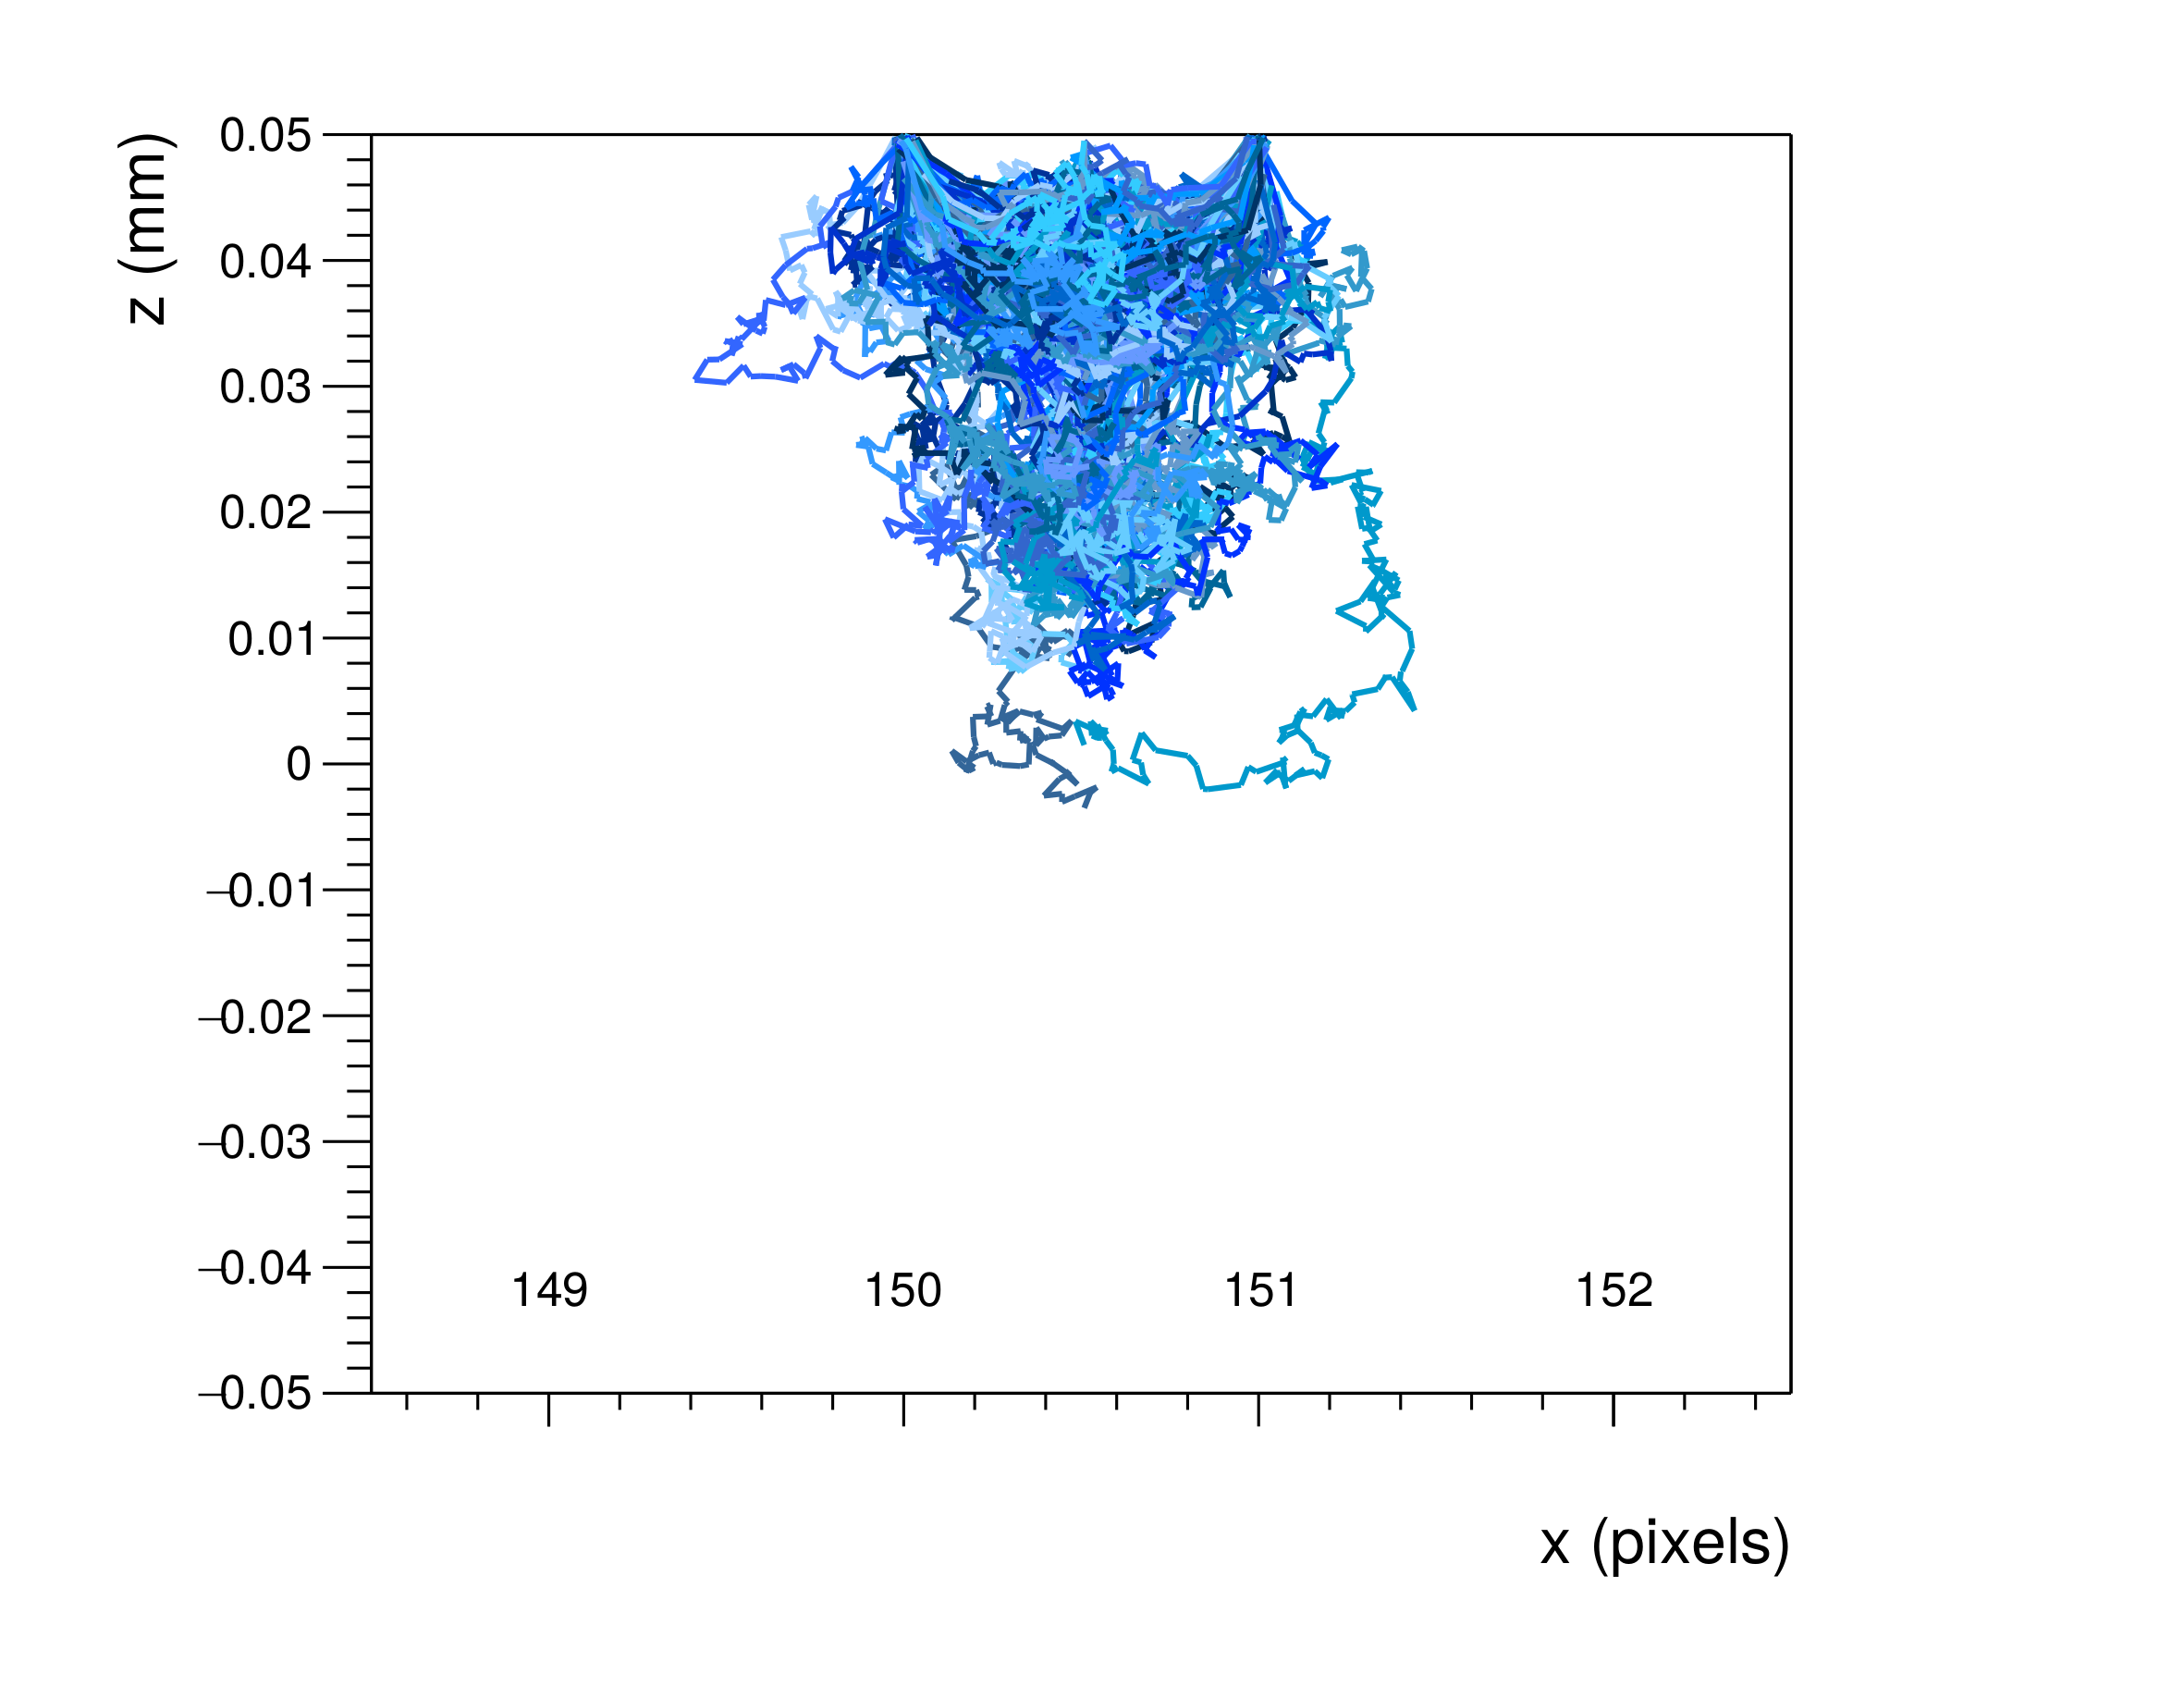
\includegraphics[width=0.7\textwidth]{linegraph_hrcmos_collected.png}
  \caption{Drift and diffusion visualization of charge carrier groups being transported through a high-resistivity CMOS silicon sensor. The plot shows the situation after an integration time of \SI{20}{\nano \second}, only charge carrier groups which reached the implant side of the sensor are drawn.}
  \label{fig:linegraph}
\end{figure}

With these settings, a graph of similar precision to the one presented in Figure~\ref{fig:linegraph} can be produced.
The required time stepping size and number of output plot steps varies greatly with the sensor and its applied electric field.
The number of charge carriers per group can be used to vary the density of lines drawn. Larger groups result in fewer lines.
\end{description}

\todo{Add more questions}
